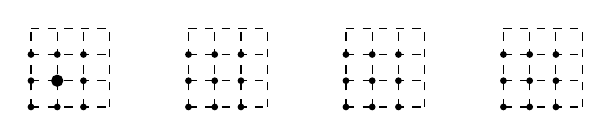
\begin{tikzpicture}[scale=1.0]
  %\draw[->,very thin] (-0.2,0.0) -- (1.2,0.0) node[below] {$x$};
  %\draw[very thin] (0.0,1.0) -- (0.0,0.0) -- (1.0,0.0);
  \pgfmathsetmacro\third{1.0/3.0}

  \draw[xstep=\third,ystep=\third,black,thin,dashed] (0.0,0.0) grid (1.0,1.0);
  \draw[black,thin,dashed] (0.0,0.0) -- (0.0,1.0);
  \foreach \x in {0,...,2} {
    \foreach \y in {0,...,2} {
        \filldraw (\x * \third,\y * \third) circle (1.0pt);
    }
  }
  \filldraw (\third,\third) circle (2.0pt);

  \draw[xstep=\third,ystep=\third,black,thin,dashed] (2.0,0.0) grid (3.0,1.0);
  \draw[black,thin,dashed] (2.0,0.0) -- (2.0,1.0);
  \foreach \x in {0,...,2} {
    \foreach \y in {0,...,2} {
        \filldraw (2.0 + \x * \third,\y * \third) circle (1.0pt);
    }
  }

  \draw[xstep=\third,ystep=\third,black,thin,dashed] (4.0,0.0) grid (5.0,1.0);
  \draw[black,thin,dashed] (4.0,0.0) -- (4.0,1.0);
  \foreach \x in {0,...,2} {
    \foreach \y in {0,...,2} {
        \filldraw (4.0 + \x * \third,\y * \third) circle (1.0pt);
    }
  }

  \draw[xstep=\third,ystep=\third,black,thin,dashed] (6.0,0.0) grid (7.0,1.0);
  \draw[black,thin,dashed] (6.0,0.0) -- (6.0,1.0);
  \foreach \x in {0,...,2} {
    \foreach \y in {0,...,2} {
        \filldraw (6.0 + \x * \third,\y * \third) circle (1.0pt);
    }
  }
\end{tikzpicture}

